% Options for packages loaded elsewhere
\PassOptionsToPackage{unicode}{hyperref}
\PassOptionsToPackage{hyphens}{url}
%
\documentclass[
]{article}
\usepackage{lmodern}
\usepackage{amssymb,amsmath}
\usepackage{ifxetex,ifluatex}
\ifnum 0\ifxetex 1\fi\ifluatex 1\fi=0 % if pdftex
  \usepackage[T1]{fontenc}
  \usepackage[utf8]{inputenc}
  \usepackage{textcomp} % provide euro and other symbols
\else % if luatex or xetex
  \usepackage{unicode-math}
  \defaultfontfeatures{Scale=MatchLowercase}
  \defaultfontfeatures[\rmfamily]{Ligatures=TeX,Scale=1}
\fi
% Use upquote if available, for straight quotes in verbatim environments
\IfFileExists{upquote.sty}{\usepackage{upquote}}{}
\IfFileExists{microtype.sty}{% use microtype if available
  \usepackage[]{microtype}
  \UseMicrotypeSet[protrusion]{basicmath} % disable protrusion for tt fonts
}{}
\makeatletter
\@ifundefined{KOMAClassName}{% if non-KOMA class
  \IfFileExists{parskip.sty}{%
    \usepackage{parskip}
  }{% else
    \setlength{\parindent}{0pt}
    \setlength{\parskip}{6pt plus 2pt minus 1pt}}
}{% if KOMA class
  \KOMAoptions{parskip=half}}
\makeatother
\usepackage{xcolor}
\IfFileExists{xurl.sty}{\usepackage{xurl}}{} % add URL line breaks if available
\IfFileExists{bookmark.sty}{\usepackage{bookmark}}{\usepackage{hyperref}}
\hypersetup{
  pdftitle={Emission Zones in London},
  pdfauthor={Finn-Henrik Barton},
  hidelinks,
  pdfcreator={LaTeX via pandoc}}
\urlstyle{same} % disable monospaced font for URLs
\usepackage[margin=1in]{geometry}
\usepackage{graphicx,grffile}
\makeatletter
\def\maxwidth{\ifdim\Gin@nat@width>\linewidth\linewidth\else\Gin@nat@width\fi}
\def\maxheight{\ifdim\Gin@nat@height>\textheight\textheight\else\Gin@nat@height\fi}
\makeatother
% Scale images if necessary, so that they will not overflow the page
% margins by default, and it is still possible to overwrite the defaults
% using explicit options in \includegraphics[width, height, ...]{}
\setkeys{Gin}{width=\maxwidth,height=\maxheight,keepaspectratio}
% Set default figure placement to htbp
\makeatletter
\def\fps@figure{htbp}
\makeatother
\setlength{\emergencystretch}{3em} % prevent overfull lines
\providecommand{\tightlist}{%
  \setlength{\itemsep}{0pt}\setlength{\parskip}{0pt}}
\setcounter{secnumdepth}{-\maxdimen} % remove section numbering

\title{Emission Zones in London}
\usepackage{etoolbox}
\makeatletter
\providecommand{\subtitle}[1]{% add subtitle to \maketitle
  \apptocmd{\@title}{\par {\large #1 \par}}{}{}
}
\makeatother
\subtitle{The impact of zoning policy on NO\(_2\) levels in Greater London}
\author{Finn-Henrik Barton}
\date{2021-06-25}

\begin{document}
\maketitle

\hypertarget{introduction}{%
\subsection{Introduction}\label{introduction}}

This blog post aims to explore the impact of the Ultra Low Emission Zone
(ULEZ) on air pollution in London. Official reports on the impact of the
ULEZ simply looked at the difference between emission in the affected
area and the outskirts of Greater London. Due to potential spatial
spillovers from the policy, I looked at re-estimating the results by
using a synthetic control group based on other metropolitan areas in the
United Kingdom. The results indicate that emission reductions from the
ULEZ are around 40\%, or 9\% higher than the official estimates made by
the Mayor of London.

\hypertarget{background}{%
\subsection{Background}\label{background}}

In 2017 it was estimated that air pollution in London was costing the
healthcare system upwards of £3.7 billion per year and resulting in
9,400 premature deaths
(\href{https://www.londoncouncils.gov.uk/node/33224}{London Councils,
2017}). Air pollution has also been found to significantly increase
crime, and impair cognition
(\href{https://www.journals.uchicago.edu/doi/full/10.1086/707127}{Bondy,
Roth, and Sage, 2012};
\href{https://www.nature.com/articles/mp201176}{Fonken et al., 2011}).
In addition to the widespread health and societal issues, reductions in
emissions from road transport will play a vital role in achieving
net-zero by 2050
(\href{https://unfccc.int/sites/default/files/resource/328_TransportDecarbonizationToolbox_TalanoaDialog.pdf}{UNFCCC,
2018}).

NO\(_2\) has been a particularly large problem in the United Kingdom,
with many urban areas failing to meet the 2010 target of
40\(\frac{\mu g}{m^3}\) per year.

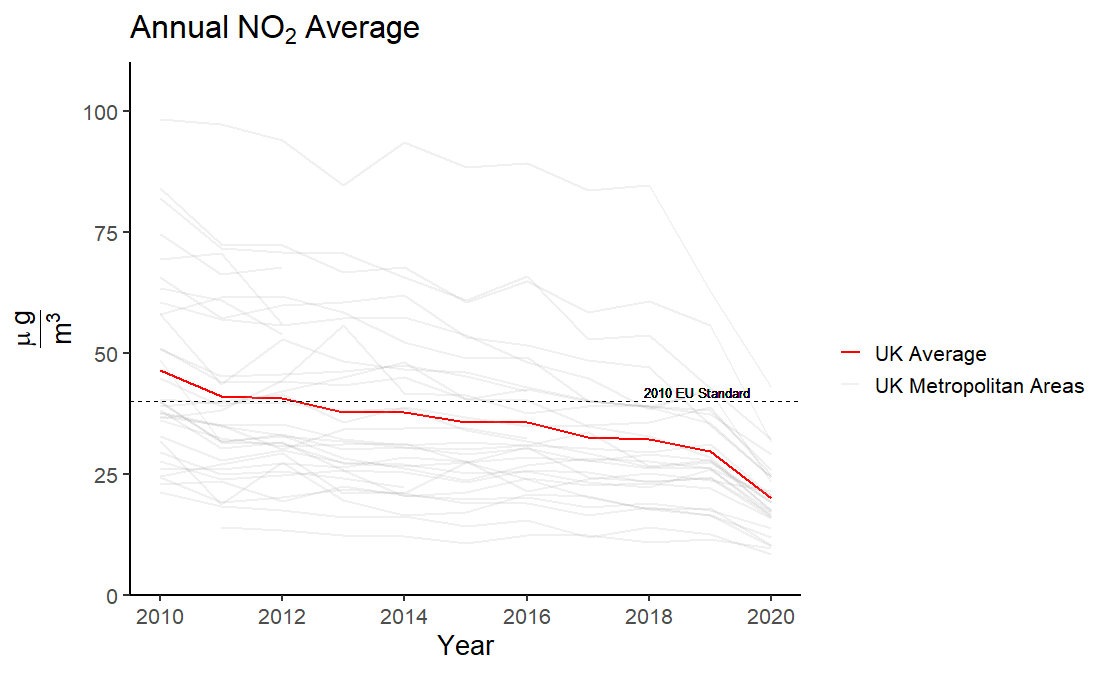
\includegraphics[width=0.8\textwidth,height=\textheight]{no2AverageUK.png}

As of July 2020, NO\(_2\) levels were still above the target emissions
set by the European Union for 2010. It wasn't until 2019 that the area
of London which is now covered by the ULEZ was able to bring the number
of annual NO\(_2\) episodes in line with the 2010 targets, where one
NO\(_2\) episode is classified as a 24 hour period where the average air
pollution levels are above 50\(\frac{\mu g}{m^3}\).

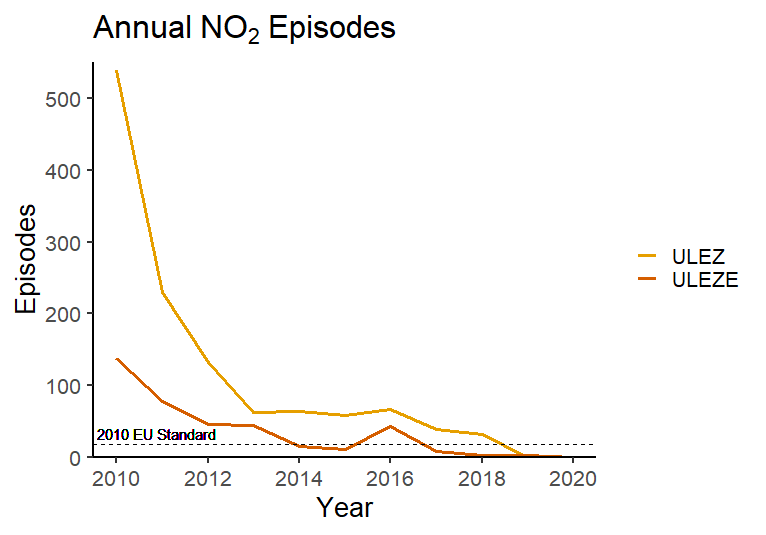
\includegraphics[width=0.8\textwidth,height=\textheight]{NO2Episodes.png}

In an attempt to combat the rising air pollution, a Toxicity-Charge
(T-Charge) was imposed in Central London in 2017. The policy applied a
£10 charge to any vehicle which was registered before 2006 which
travelled through the London congestion zone. Two months later on the
1st of January, 2018, the transition towards an Ultra Low Emission Zone
(ULEZ) started. From the start of the transition period, all new taxis
and private hire vehicles should be zero emission capable. On the 8th of
April, 2019, the ULEZ replaced the T-Charge, imposing a £12.50 charge
for most existing vehicles, and £100 for heavy vehicles. As of the 25th
of October 2021, there will be a new Ultra Low Emission Zone Expansion
(ULEZE), which will extend to London's North and South circular roads.

\includegraphics{LondonSites.jpg}

\hypertarget{how-do-we-calculate-the-impact}{%
\subsection{How do we calculate the
impact?}\label{how-do-we-calculate-the-impact}}

One of the main difficulties when assessing the efficacy of emission
zoning policy is the ability to find a suitable control group. Due to
spatial spillovers, regions within close proximity to where the policy
was enacted are often indirectly impacted by the policy. Consequently,
comparing the changes in emissions between an effected area compared to
surrounding areas will likely lead to biased estimates.

Another way to think of these spillovers is to consider what happens
when a rock(policy) is thrown in a lake. When the rock hits the water it
creates a large initial splash(treatment effect), and
ripples(spillovers) follow. The further we move away from where the rock
landed, the smaller the ripples will become. Consequently, if we are
interested in measuring the height of the splash relative to the normal
level of the lake, we want to compare the size of the splash to another
area far away from where the rock landed. Note that if we chose a
location which was too close, we may observe a value which is either at
the peak or trough of the ripples, hence biasing our estimates.
Furthermore, we also need to make sure that there were no other rocks
thrown in the lake at the point we are using as our comparison point, as
this would also lead to skewed results.

What this means for assessing the policy efficacy is that we would want
to find a control group which is highly unlikely to be affected by the
policy, but hopefully still follow the same path as the affected area if
the policy was not put in place. A common way for checking whether our
control group is likely to follow the same path as our treatment in the
absence of the policy, is by checking whether they had parallel trends
prior to the policy intervention. Looking at the change in the
difference between these two groups before and after the policy
implementation, we can get an indication of the average treatment
effect.

\hypertarget{impact-of-the-zoning-policies}{%
\subsection{Impact of the zoning
policies}\label{impact-of-the-zoning-policies}}

In order to assess the change in air pollution, daily air pollution data
from 150 Automatic Urban and Rural Network (AURN) sites all over the UK
were analysed. Air pollution values were then deseasonalised and
aggregated at a monthly rate. The data provides reasonable estimates of
air pollution for 28 metropolitan areas. Taking a weighted average of
other metropolitan areas in the United Kingdom, we can create a
``synthetic'' control group which satisfy the parallel trend assumption.
In an effort to minimise the spatial spillovers Greater London and
neighbouring counties were excluded. Furthermore, any metropolitan areas
which implemented policies to reduce air pollution between 2010 and July
2021 were also excluded as potential control groups. Although we can
never be certain that there are no spillovers, by only selecting
metropolitan areas which are outside of a reasonable commuting time to
the ULEZ, the spillovers are hopefully minimised.

the Mayor of London released two reports
{[}\href{https://www.london.gov.uk/sites/default/files/ulez_six_month_evaluation_report_final_oct.pdf}{2019},
\href{https://www.london.gov.uk/sites/default/files/ulez_ten_month_evaluation_report_23_april_2020.pdf}{2020}{]}
summarising the impact of the ULEZ on air pollution, and concluded that
the zoning policy reduced roadside NO\(_2\) by 31\% and 37\%
respectively in the two reports. The reports measured changes in
roadside levels between ULEZ monitoring stations and monitoring stations
located at the periphery of Greater London. Comparing the results from
the latest report from the Mayor of London to the results from the
synthetic control method indicates the policy was effective at reducing
roadside NO\(_2\) emission by 40.5\% as of January 2020.

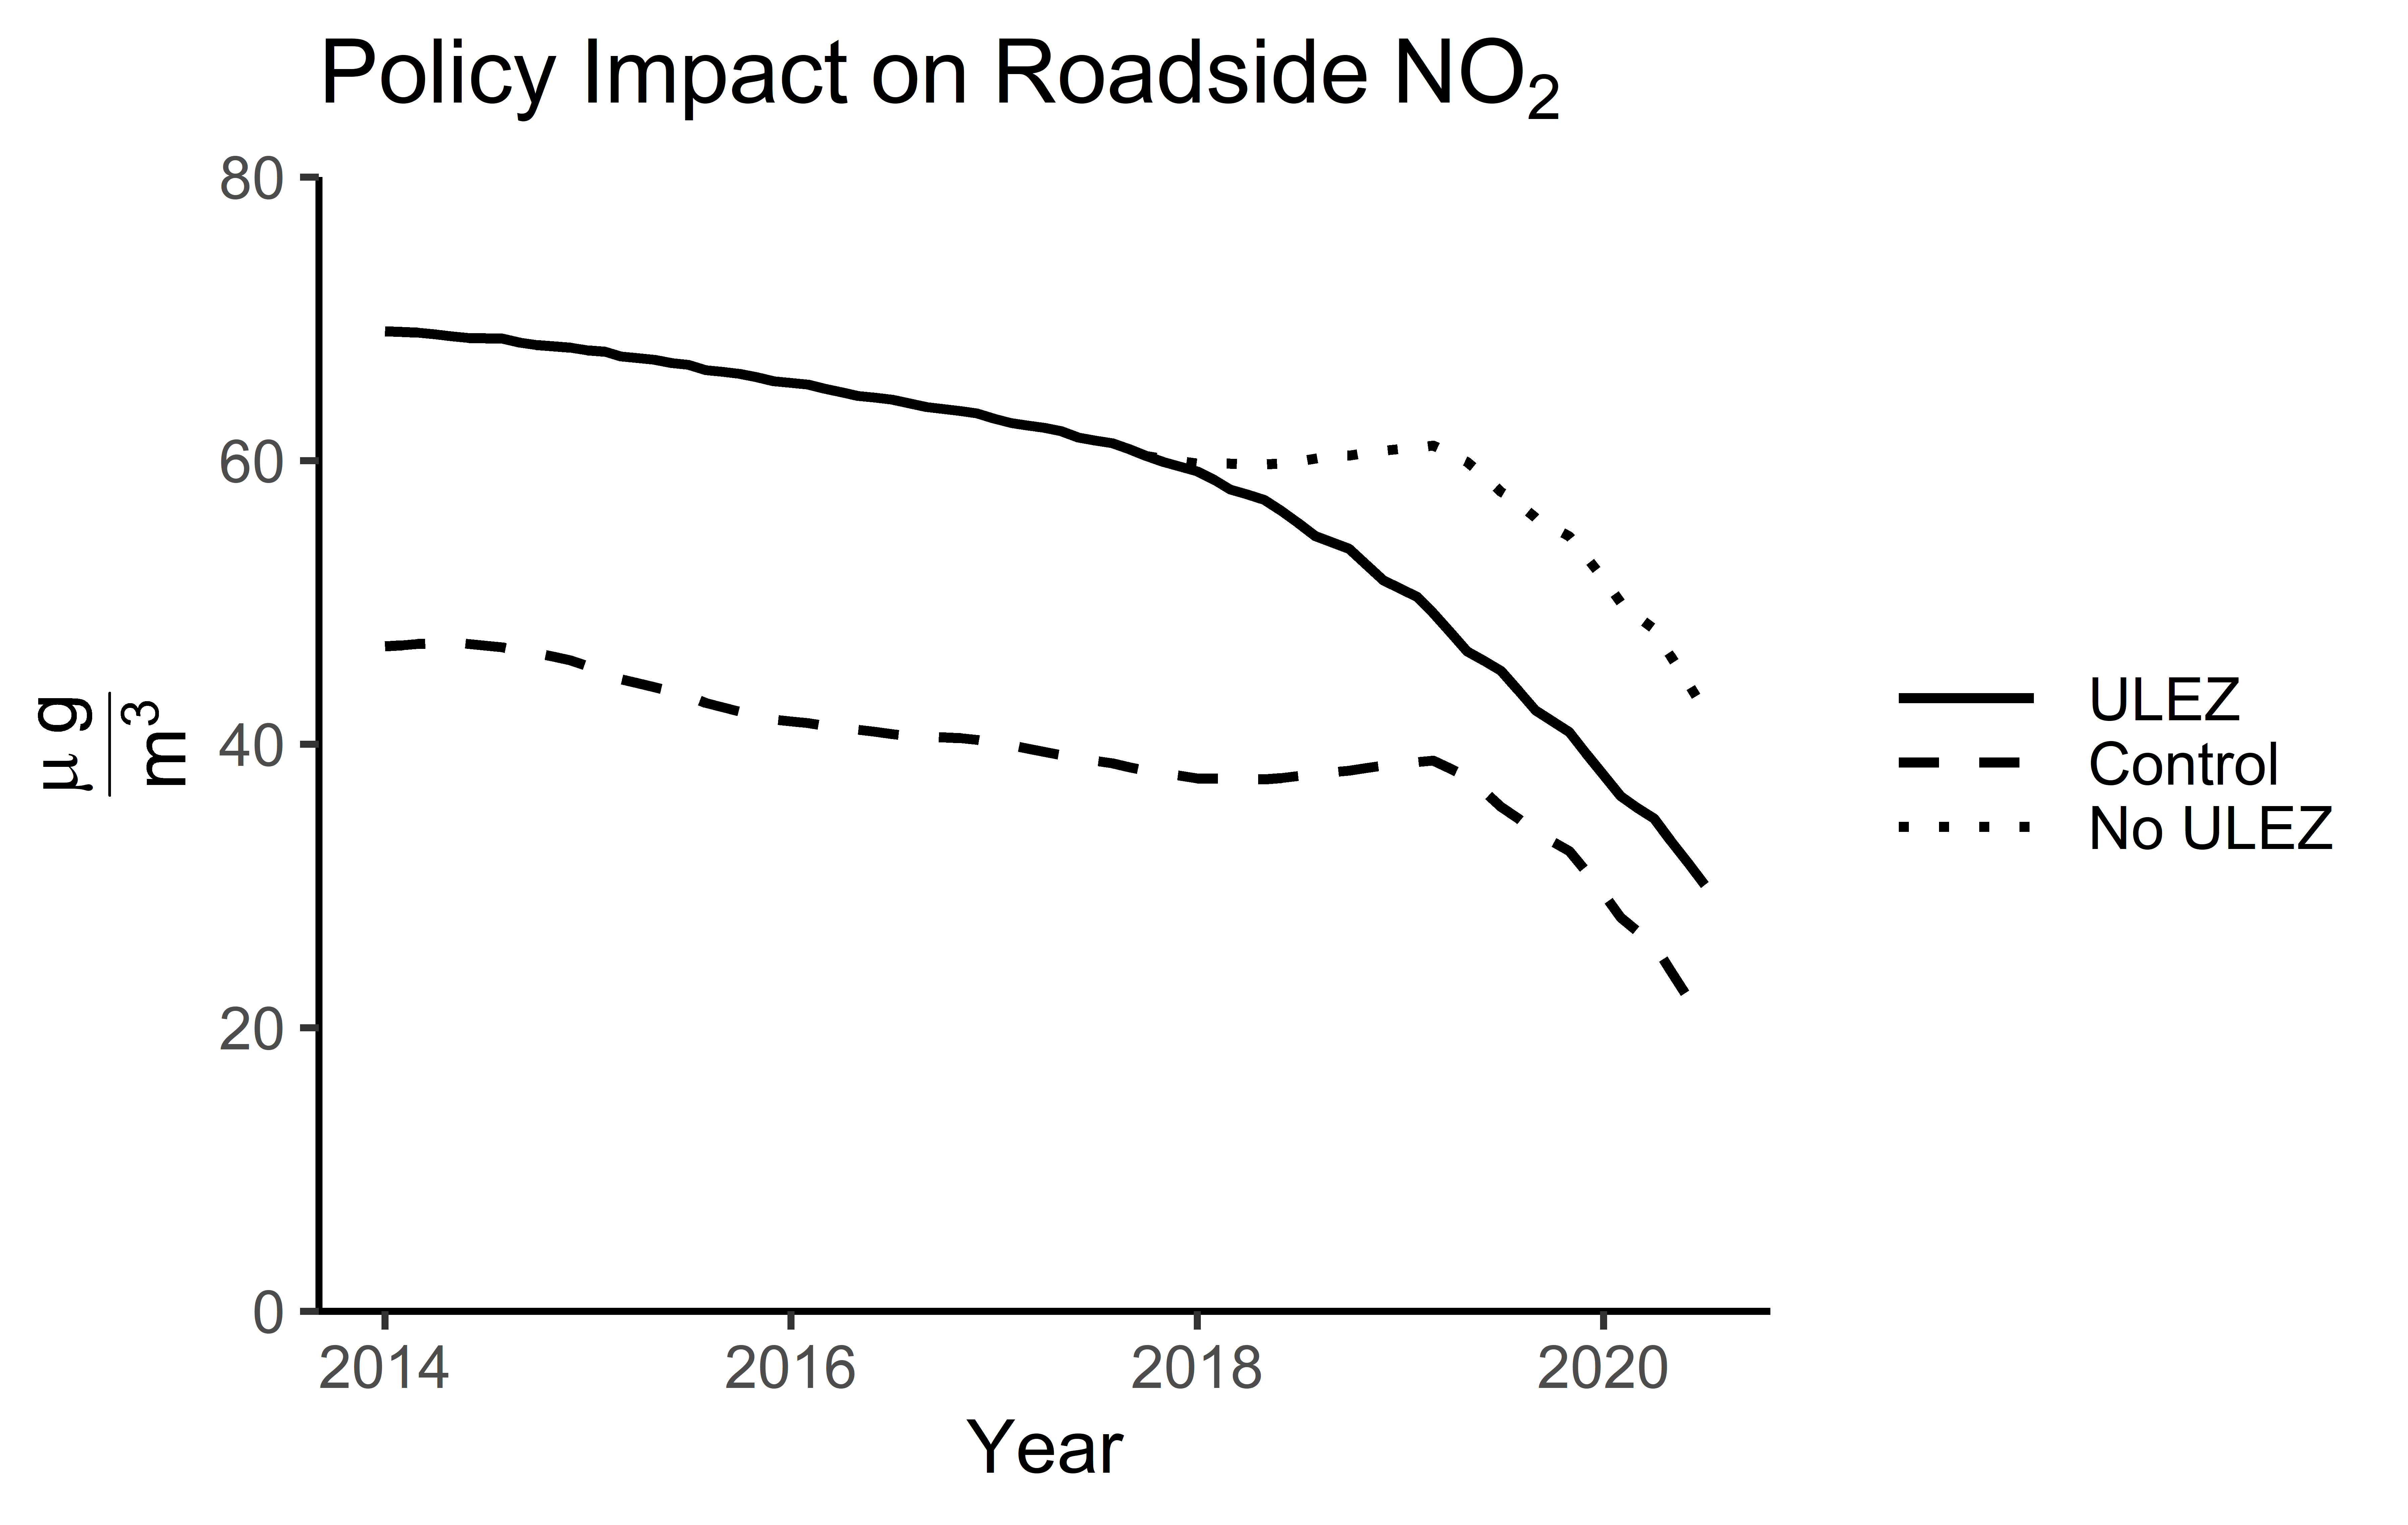
\includegraphics{NO2_DiD.png}

The sharp fall seen in the control group in 2019 can be observed in
almost all metropolitan areas. This drop was likely due to the unveil of
the
\href{https://www.gov.uk/government/publications/clean-air-strategy-2019/clean-air-strategy-2019-executive-summary}{Clean
Air Strategy} which laid out a plan for reducing air pollution in the UK
by 2020 and 2030.

\hypertarget{concluding-remarks}{%
\subsection{Concluding remarks}\label{concluding-remarks}}

The purpose of this blog post was to explore the use of synthetic
controls in a spatial setting, looking at a case-study of the emission
zoning policies in London. After accounting for spatial spillovers, it
is likely that the Ultra Low Emission Zone reduced emissions in Central
London by up to 40.5\%, which is 9\% greater than the official estimates
by the Mayor of London.

This being said, the analysis is far from perfect. Firstly, in the data
there are only 150 monitoring stations, this means that the number of
monitoring stations per metropolitan area is very low. Consequently, the
air pollution data may not accurately represent all metropolitan areas.
Secondly, caution should be exercised when interpreting these results as
causal. The parallel trend assumption did not hold for any other air
pollutants than NO\(_2\). One explanation from this is that using other
metropolitan areas in the UK as a control group may not be a good
representation of London, as it is often viewed as its own microcosm
within the UK.

To conclude, I would say that the results do indicate that that the ULEZ
was effective in reducing NO\(_2\) concentrations in Central London.
Furthermore, the results imply that the effect may be greater than
official estimates due to spatial spillovers. With the Expansion of the
ULEZ in October 2021, it will be exciting to see the impact on urban air
pollution. Luckily, it does seem like we are moving towards greener and
cleaner urban spaces.

\end{document}
